
\subsection*{Change of Basis Example}

%%%Insert this to get the typewriter font so it looks like a real movie script
{\ttfamily
\fontdimen2\font=0.4em
\fontdimen3\font=0.2em
\fontdimen4\font=0.1em
\fontdimen7\font=0.1em
\hyphenchar\font=`\-


\hypertarget{scripts_diagonalization_basis}{This video} returns to 
the example of a barrel filled with fruit
\begin{center}
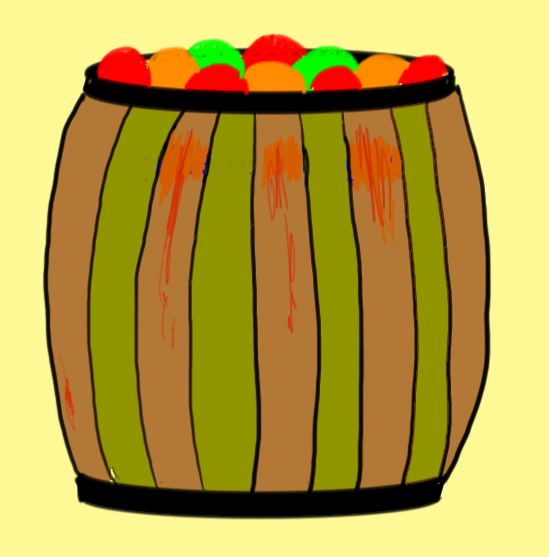
\includegraphics[scale=.3]{\diagPath/barrel.jpg}
\end{center}
as a demonstration of changing basis.

Since this was a linear systems problem, we can try to represent what's in the barrel using a vector space. The first representation was the one
where $(x,y)=(\mbox{apples},\mbox{oranges})$:
\vspace{2mm}
\begin{center}
\begin{tikzpicture}[domain=0:4]
    \draw[->] (-0.2,0) -- (4.2,0) node[right] {$\mbox{Apples}$};
    \draw[->] (0,-1.2) -- (0,4.2) node[above] {$\mbox{Oranges}$};
    \draw[->] (0,0) -- (2,3) node[anchor=south east] {$(x,y)$};
\end{tikzpicture}
\end{center}
Calling the basis vectors $\vec e_1:=(1,0)$ and $\vec e_2:=(0,1)$, 
this representation would label what's in the barrel by a vector 
\[
\vec x: = x \vec e_1 + y\vec e_2 = \begin{pmatrix}\vec e_1 & \vec e_2\end{pmatrix}\begin{pmatrix}x \\ y\end{pmatrix}\, .
\]
Since this is the method ordinary people would use, we will call this the
``engineer's'' method!


But this is not the approach nutritionists would use. They would note the amount of sugar and total number of fruit~$(s,f)$:
\begin{center}
\begin{tikzpicture}[domain=0:4]
    \draw[very thin,color=gray] (-0.1,-1.1) grid (3.9,3.9);
    \draw[->] (-0.2,0) -- (4.2,0) node[right] {sugar};
    \draw[->] (0,-1.2) -- (0,4.2) node[above] {fruit};
    \draw[->] (0,0) -- (2,3) node[anchor=south east] {\scalebox{.75}{${ (s,f)}$}};
\end{tikzpicture}
\end{center}
WARNING: To make sense of what comes next you need to allow for the possibity of a negative amount of fruit or sugar. This would be just like a bank, where if money is owed to somebody else, we can use a minus sign.

The vector $\vec x$ says what is in the barrel and does not depend which mathematical description is employed. The way nutritionists label $\vec x$ 
is in terms of a pair of basis vectors $\vec f_1$ and $\vec f_2$:
\[
\vec x=s \vec f_1 + f \vec f_2=\begin{pmatrix}\vec f_1 & \vec f_2\end{pmatrix}\begin{pmatrix}s \\ f\end{pmatrix}\, .
\]

Thus our vector space now has a bunch of interesting vectors:
\begin{center}
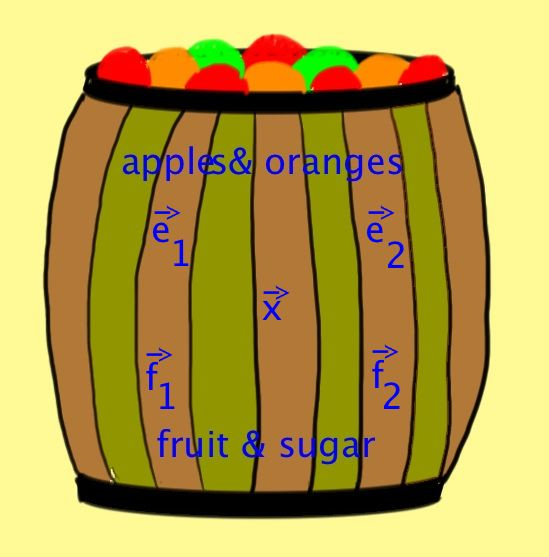
\includegraphics[scale=.3]{\diagPath/barrel3.jpg}
\end{center}
The vector $\vec x$ labels generally the contents of the barrel. The 
vector $\vec e_1$ corresponds to one apple and one orange. The vector $\vec e_2$ is one orange and no apples. The vector $\vec f_1$ means one unit of sugar and zero total fruit (to achieve this you could  lend out some apples and keep a few oranges). Finally the vector $\vec f_2$ represents a total of one piece of fruit and no sugar.

You might remember that the amount of sugar in an apple 
is called $\lambda$ while oranges have twice as much sugar as apples.
Thus
\[
\left\{
\begin{array}{l}
s=\lambda\, (x+2y)\\
f=x+y\, .
\end{array}
\right.
\]
Essentially, this is already our change of basis formula, but lets play around and put it in our notations.
First we can write this as a matrix
\[
\begin{pmatrix}s\\f\end{pmatrix}=
\begin{pmatrix}\lambda & 2\lambda \\1 & 1
\end{pmatrix}
\begin{pmatrix}x\\y\end{pmatrix}\, .
\]
We can easily invert this to get
\[
\begin{pmatrix}x\\y\end{pmatrix}
=
\begin{pmatrix}-\frac1\lambda & 2\\ \frac1\lambda & -1
\end{pmatrix}
\begin{pmatrix}s\\f\end{pmatrix}\, .
\]
Putting this in the engineer's formula for $\vec x$ gives
\[
\vec x = 
\begin{pmatrix}\vec e_1 & \vec e_2\end{pmatrix}
\begin{pmatrix}-\frac1\lambda & 2\\ \frac1\lambda & -1
\end{pmatrix}
\begin{pmatrix}s\\f\end{pmatrix}
=
\begin{pmatrix}-\frac1\lambda\big(\vec e_1 - \vec e_2\big) &
2\vec e_1-2\vec e_2\end{pmatrix}
\begin{pmatrix}s\\f\end{pmatrix}\, .
\]
Comparing to the nutritionist's formula for the same object $\vec x$ we learn that
\[
\vec f_1 = -\frac1\lambda\big(\vec e_1 - \vec e_2\big)\quad \mbox{and}\quad
\vec f_2=2\vec e_1-2\vec e_2\, .
\]
Rearranging these equation we find the change of base matrix $P$ from the engineer's basis to the nutritionist's basis:
\[
\begin{pmatrix}\vec f_1 & \vec f_2\end{pmatrix}
=
\begin{pmatrix}\vec e_1 & \vec e_2\end{pmatrix}
\begin{pmatrix}-\frac1\lambda & 2\\ \frac1\lambda & -1
\end{pmatrix} =:\begin{pmatrix}\vec e_1 & \vec e_2\end{pmatrix} \, P\, .
\]
We can also go the other direction, changing from the nutritionist's basis to the  engineer's basis
\[
\begin{pmatrix}\vec e_1 & \vec e_2\end{pmatrix}
=
\begin{pmatrix}\vec f_1 & \vec f_2\end{pmatrix}
\begin{pmatrix}\lambda & 2\lambda \\ 1 & 1
\end{pmatrix} =:\begin{pmatrix}\vec f_1 & \vec f_2\end{pmatrix} \, Q\, .
\]
Of course, we must have 
\[
Q=P^{-1}\, ,
\]
(which is in fact how we constructed $P$ in the first place).

Finally, lets consider the very first linear systems problem, where you were given that there were 27 pieces of fruit in total and twice as many oranges as apples. In equations this says just
\[
x+y=27\quad \mbox{and} \quad 2x-y=0\, .
\]
But we can also write this as a matrix system
\[
MX=V
\]
where 
\[
M:=\begin{pmatrix} 1 & 1 \\ 2 & -1 \end{pmatrix}\, ,\qquad
X:=\begin{pmatrix}x \\y \end{pmatrix}\, \,\qquad
V:=\begin{pmatrix}0 \\ 27\end{pmatrix}\, .
\]
Note that 
\[
\vec x = \begin{pmatrix}\vec e_1 & \vec e_2\end{pmatrix}\, X\, .
\]
Also lets call \[ \vec v:= \begin{pmatrix}\vec e_1 & \vec e_2\end{pmatrix}\, V\, .\]
Now the matrix $M$ is the matrix of some linear transformation $L$ in the basis of the engineers.
Lets convert it to the basis of the nutritionists:
\[
L\vec x = L \begin{pmatrix}\vec f_1 & \vec f_2\end{pmatrix}
\begin{pmatrix} s \\  f\end{pmatrix}
= L \begin{pmatrix}\vec e_1 & \vec e_2\end{pmatrix} P \begin{pmatrix} s \\  f\end{pmatrix}
= \begin{pmatrix} \vec e_1 \\ \vec e_2\end{pmatrix} M P \begin{pmatrix} s \\  f\end{pmatrix}\, .
\]
Note here that the linear transformation on acts on {\itshape vectors} -- these are the objects we have written with a $\vec{}$ sign on top of them. It does not act on columns of numbers!

We can easily compute $MP$ and find
\[
MP=\begin{pmatrix} 1 & 1 \\ 2 & -1 \end{pmatrix}\begin{pmatrix}-\frac1\lambda & 2\\ \frac1\lambda & -1
\end{pmatrix}
=\begin{pmatrix}0& 1\\ -\frac3\lambda & 5
\end{pmatrix}\, .
\] 
Note that $P^{-1}MP$ is the matrix of $L$ in the nutritionists basis, but we don't need this quantity right now.

Thus the last task is to solve the system, lets solve for sugar and fruit. 
We need to solve
\[
MP\begin{pmatrix} s \\  f\end{pmatrix}
=\begin{pmatrix}0& 1\\ -\frac3\lambda & 5
\end{pmatrix}
\begin{pmatrix} s \\  f\end{pmatrix}
=\begin{pmatrix}27\\0\end{pmatrix}
\, .
\]
This is solved immediately by forward substitution (the nutritionists basis is nice since it directly gives $f$):
\[
f=27\quad \mbox{and} \quad s= 45\lambda\, .
\]

} % Closing bracket for font

%\newpage
